\section{Algorithm for near duplicate detection}
\label{section:luciv}

In the section the improved version of Luciv et.al. algorithm~\cite{luciv2019interactive} is presented.
The utilization of semi-local sequence alignment algorithms in algorithm phases improves overall time complexity.
%% We now describe an improved version of  by utilizing a \emph{semi-local sa} solution.
%% Then we present proof that improved version preserves completnesess property.
%% It is achieved by imitating all phases of the algorithm. 
It is also proved that the improved algorithm preserves all advantages of the initial one stated at~\cite{luciv2019interactive} such as search completeness.

\subsection{Algorithm description}
As the base one (see section~\ref{sec:lucivalgo} and~\ref{Luciv}), the presented algorithm consists of three sequential phases.
%Moreover, each step of the presented algorithm imitates the corresponding step of the base one.
Aldorithm pseudocode is presented at Algorithm~\ref{alg:patternMathing1}.
% As the base one, the presented algorithm comprises three phases.

At the first phase (lines 1-3) semi-local sa problem is solved for pattern $p$ against the whole text $t$.
This solution provides access to the string-substring matrix $H^{str-sub}_{p,t}$ which allows performing fast queries of \emph{sa} score for pattern $p$ against every substring of text $t$.
Then, we construct matrix $M$ by applying transposition and inverse operation implicitly on $H^{str-sub}_{p,t}$:
$$M[j,i]:= -H^{str-sub}_{p,t}[i,j].$$
Note, transposition operation preserves (anti) Monge property whereas inverse operation transforms anti-Monge matrix into the Monge one and vice versa. 
Thus, $M$ is a Monge matrix.

The second phase comprises several steps (lines 4--6).
First, we want to get for each substring with length exactly $L_{w}$ in  $t$ its alignment score against pattern $p$ where $k \in (\frac{1}{\sqrt{3}},1]$.
Second, for each substring $w$ of size $L_{w}$ in text $t$ that meets criteria on similarity with given threshold $-k_{di}$ the following should be done.
The longest substring  most similar to pattern $p$ should be taken.
it could be done by processing the diagonal 
matrix $M$ with width $c:= \frac{|p|}{k} - |p|*k = |p|(\frac{1}{k} - k)$ (Fig. \ref{M2}).

The third phase (lines 7--11) is the same as in the base algorithm.

 
\begin{figure}
	\centering
   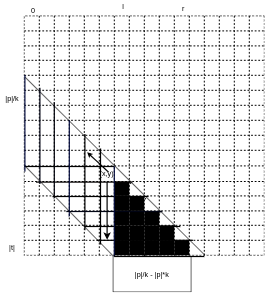
\includegraphics[width=0.4\columnwidth]{figures/M2.png}
   \caption{LOL}\label{M2}
\end{figure}




\begin{algorithm}[!t]
\caption{PATTERN BASED NEAR DUPLICATE
SEARCH ALGORITHM VIA SEMI-LOCAL SA}
\label{alg:patternMathing1}
Input: pattern $p$, text $t$, similiarity measure $k \in  [ \frac{1}{\sqrt{3}} ,1  ]$\\
Output: Set of non-intersected clones of pattern $p$ in text $t$
\begin{equation}
    k_{di}=|p|*(\frac{1}{k}+1)(1-k^2)
\end{equation}
\begin{equation}
 L_{w} = \frac{|p|} {k}
\end{equation}
\begin{equation}
  w = |p|(\frac{1}{k} - k)
\end{equation}
Pseudocode:
\begin{algorithmic}[1]
\STATE{$W = semilocalsa(p,t)$}
\COMMENT{1st phase}
\STATE{$H^{str-sub}_{p,t} = semilocalsa(p,t).stringSubstringMatrix$}
\STATE{$M[j,i] = -H^{str-sub}_{p,t}[i,j]  $}
\STATE{$sufixes = processDiagonal(M,L)$}
\COMMENT{2d phase}
\STATE{$W_2 = SuffixMaxForEachWindow(sufixes,L_{w})$}
%% \STATE{$filter(W_2,k_{di})$}
\STATE{ $W_3 = UNIQUE(W_2)$}
\COMMENT{3rd phase unchanged}
\FOR{$w \in W_3$}
\IF{$\exists w^{'} \in W_3:w \subset w^{'} $}
\STATE{ $remove$ $w$ $from$ $W_3$}
\ENDIF
\ENDFOR
\RETURN $W_3$
\end{algorithmic}
\end{algorithm}

\begin{theorem}
Algorithm \ref{alg:patternMathing1} runs in $max(O(|t|*|p|),\ O(|t| * \log |t|))$ time with $O( |t| \log |t|)$ additional space where $p$ is pattern, $t$ is text, $|p| \leq |t|$, and $v=O(1)$ where $v$ is denominator of normalized mismatch score for semi-local sa $w_{normalized} = (1,\frac{\mu}{v},0)$.
\end{theorem}
\begin{proof}
  For each phases of algorithm we provide it's time and space bounds.
  
\emph{First phase.}
We store solution $H$ of \emph{semi-local sa} by decomposing it to permutation matrix $P$ of size $O(v*|t| \times v*|t|)$ (lines 1-3, Theorem~\ref{decomposition}).
The permutation matrix can be stored via two permutations of size $v*|t|$ for columns and rows.
It is simply two lists of size $v*|t|$.
Then, for random access query in specific position $(i,j)$ of matrix $H$ one need to check how many points are dominated by $H [i,j]$.
It can be done by checking all points of permutation matrix and requires $O(v * |t|)$ steps.
Thus, the total time and space complexity of the first phase are $O(v *|p| * |t|)$ (time needed to solve semi-local sa) and $O(v*|t|)$ respectively.
Given $v=O(1)$ we have $O(|p| * |t|)$ and $O(|t|)$ respectively.

\emph{Second phase}.
For the sake of clarity, we omit $k$ factor in algorithm analysis since $k$ is just a constants within interval $(\frac{1}{\sqrt{3}},1]$.

%We proceed diagonal M as follows (\ref{M2}).
First, we query elements that lie in the diagonal that represent
substrings of size $L_{w}=\frac{|p|}{k}$ (to step onto $(0,|p|/k)$ cell we need to perform one orthogonal range query).
We denote them by $lstW$.
Since we can use proposition~\ref{incremental} to access
adjacent elements 
the total complexity of this step is $O(|t|)$.
The total amount of querying cells is $O(|t|)$. 
Second, we again process matrix M.
More precisely, we process the diagonal of width $O(\frac{|p|}{k}-|p|*k)=O(|p|)$ that corresponds to all substrings with size in  $I=[|p|*k, \frac{|p|}{k}]$ interval (on Fig. \ref{M2} it is  trapezoid).
Note, that the bold triangle in Fig  \ref{M2} corresponds to the set of substrings with sizes in the interval $I$ that contains in the last substring with size $L_{w}$ of text $t$.
During processing each triangle we  additionally store list $longestForRow$ of size $\frac{|p|}{k}-|p|k$ that contains
for each row (represent prefix) the suffix that is most similar to pattern $p$ for given window (triangle on Fig. \ref{M2}).
This list updated every time when we shift triangle by one symbol step ($(x,y)\rightarrow (x-1,y-1)$).
Thus, to get the longest substring that most similar to pattern $p$ for the given window we simply need
to check $longestForRow$. 
Thereby, we proceed as follows.
We check that the current window meets criteria
on similarity (it is just lookup to list $lstW$)
If so, then we find maximal substring among all associated with the current window (triangle) by checking $O(|p|)$ elements of $longestForRow$ and save it to set $W_{2}$ as described above.

Thus, the processing of each column of trapezia requires at most $O(|p|)$ time. The total amount of columns is $(|t|)$
Total time complexity of this phase is $O(|t||p|)$.
The space complexity of this phase is $O(|p|+|t|)=O(|t|)$ at most.

\emph{Third phase}.
The third phase remains unchanged, thus have the same time and space bounds as in the base algorithm case.
Note, it possible to perform this phase in-place during the second phase which speedups the algorithm, i.e decreases space and time complexity to $O(|t|)$ and $O(|t|*|p|)$ respectively.
The third phase can be approximated as $O(|t| * log|t|)$ for both space and running time complexity.

Thus, the total alforithm running time is $max(O(t * p),\ O(t * \log t))$ while space complexity is $O(t * \log t)$.
\end{proof}

\begin{theorem}
Algorithm \ref{alg:patternMathing1} with scoring scheme $w = (0,-2,-1)$ preserves completnesses property of algorithm~\cite{luciv2019interactive} and has running time and space complexity $max(O(t*p),\ O(t* \log t))$ and $O(t *  \log t)$  respectively.
\end{theorem}

\begin{proof}
Edit distance in the base algorithm~\cite{.} may be expressed as sequence alignment with following scoring scheme: 
$$w_{sa}=(w_{+},w_{0},w_{-}) = (0,-2,-1).$$

First, to get intial edit score we need to apply inverse operation:
$$editscore(a,b) = -sa(a,b,w_{sa}).$$
Next, $w_{sa}$ may be normalized using normalization~\ref{weightNormalization}:
$$(0, -2, -1) \rightarrow (1,\frac{\mu=0}{v=1}, 0).$$
Thus, $d_{di} \leq k_{di}$ is the same as $sa \geq -k_{di}$.

Second, let's carefull review phases 1 and 2 of given algorithms.
The base algorithm passes through the text with a sliding window to detect those fragments of size $L_{w}$ which have edit score above given threshold $k_{di}$.
Then within these fragments algorithm detects longest suffixes that are most similar to pattern $p$ with size within interval $I=[pk,\ L_{w}]$.
The presented improved algorithm proceeds in a very similar way but, informally, phases are swapped.
First, it detects the longest suffixes with size in interval $I$ for each prefix of the text.
Then, it proceeds in such way that for each window of size $L_{w}$ that has alignment score with pattern $p$ below given threshold $-k_{di}$  the longest suffix most similar to $p$ is detected.
Due to \todo{formula~\ref{editsa}} results of the second phases of the algorithms are equal.
The third phase remains unchaned in the presented algorithm.
%% Thus, the presented algorithm preserves completeness.
Thus, the presented algorithm is complete.
For $w = (0,-2,-1)$, $v=1$ and algorithm running time and space complexity are as claimed.
%% For given $w = (0,-2,-1)$ we have $v=1$ then wehave running time as claimed.
\end{proof}

%At first algorithm \ref{luciv} pass through text $t$ with sliding window to detect those fragments which has similarity abobe given threhsold $k_{di}$ with size $\frac{p}{k}$.
%Then within these fragments algorithm detects longest suffixes most similar to pattern $p$ with size within  $pk...\frac{p}{k}$ interval.
%That how $A_1$ constucted.
%
%T%he second algorithm \ref{alg:patternMathing1} proceed in similar way but it first .
 .
%$Then filtering is perfomed in that way that only$
%That how $A_1$ constucted.
%those lonh suffices  left 
 %for those windows of size $\frac{p}{k}$ the longest suffix is left.

%T%%hus, $A_1=A_2$  by resulting equivalence of construction. 

